\section{ERC-SVD} \label{ER-SVD_method}

\begin{figure}[ht]
    \centering
    \includegraphics[width=\textwidth]{CPAL-2025-template/a_figures/ressvd_framework.pdf}
    \caption{The overall framework of ERC-SVD, and comparison with other methods. The last $k$ layers are selected through \textbf{partial-layer compression} and compressed using \textbf{residual compensation} with calibration data. 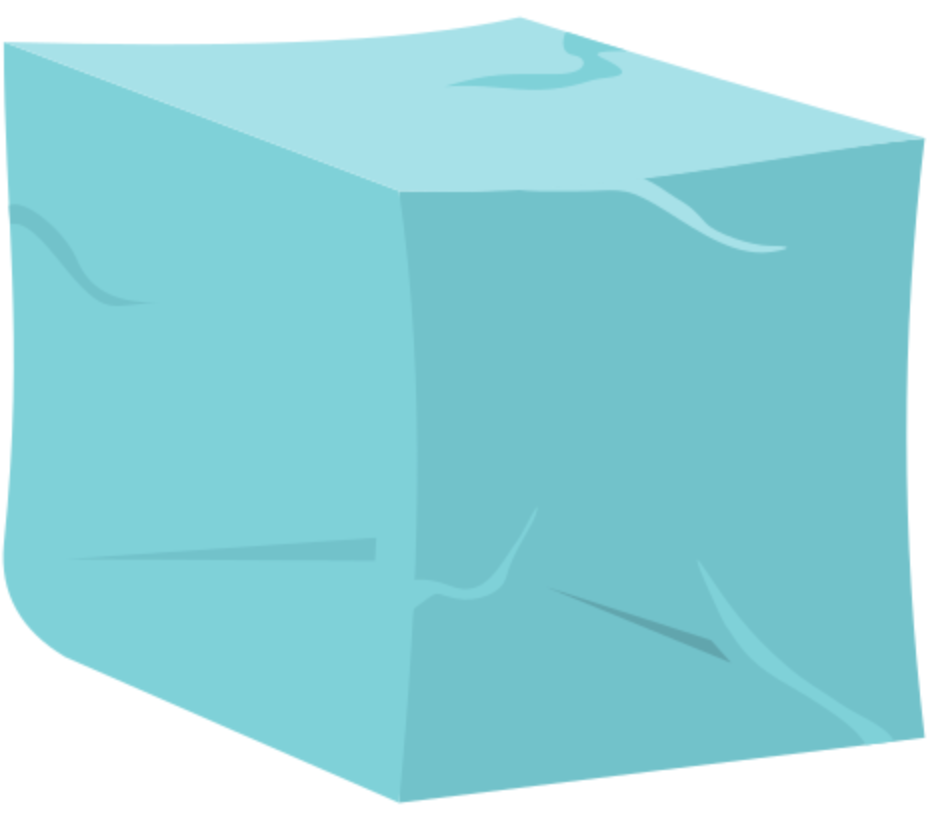
\includegraphics[height=0.8em]{CPAL-2025-template/a_figures/ice.png} denotes these layers remain intact, while 
\includegraphics[height=1em]{CPAL-2025-template/a_figures/fire.png} denotes these layers are replaced by low-rank approximations. The overall compression ratio is $R_o$, for ERC-SVD, the first $(N-k)$ layers stay unchanged, and the layer compression ratio $R_l$ for last $k$ layers is $(N \cdot R_o)/k$.} \label{ER-SVD_framework}
\end{figure}

The framework of ERC-SVD is illustrated in Figure~\ref{ER-SVD_framework}. 
We first perform SVD to compress the last few layers of the model, while ensuring that the overall compression ratio is satisfied, and compute the corresponding residual matrix. 
A second SVD is then applied to the residual matrix to obtain its low-rank approximation.
The two truncated matrices are subsequently combined to construct the final compressed weight matrices.
Compared with other methods~\cite{yuan2023asvd,wang2024svd,wang2024basis,li2025adasvd}, we utilize the residual matrix during the truncation process to compensate for the truncation loss.
In Section~\ref{sec_rc}, we first provide a detailed description of how \textbf{residual compensation} effectively works. 
Subsequently, in Section~\ref{sec_plc}, we explain the benefits of \textbf{partial-layer compression} in mitigating error propagation. The pseudocode of ERC-SVD is shown in Algorithm~\ref{alg_ER-SVD}, with the pseudocode for residual compensation and partial-layer compression provided in Algorithm~\ref{alg_rc} and Algorithm~\ref{alg_plc}, respectively.

\subsection{Residual Compensation for SVD Truncation}\label{sec_rc}
\paragraph{Preliminaries for SVD.} SVD-based compression methods apply SVD to the original weight matrix $\boldsymbol{W}\in\mathbb{R}^{m\times n}$, discarding the smallest singular values to obtain its low-rank approximation $\boldsymbol{W}_r$:
\begin{align}
   \boldsymbol{W} = \boldsymbol{U}\boldsymbol{\Sigma} \boldsymbol{V}^T \approx \boldsymbol{U}_r\boldsymbol{\Sigma}_r\boldsymbol{V}_r^T = \boldsymbol{W}_r\;,r < \min(m,n),
\end{align}
where $\boldsymbol{U}_r\in\mathbb{R}^{m\times r}$ and $\boldsymbol{V}_r^T\in\mathbb{R}^{r\times n}$ are composed of the top-$r$ left and right singular vectors, respectively, and $\boldsymbol{\Sigma}_r\in\mathbb{R}^{r\times r}$ is a diagonal matrix containing the corresponding singular values. 
Following prior post-training SVD-based works~\cite{yuan2023asvd,wang2024svd}, the optimization objective for SVD truncation in LLMs can be formulated as:
\begin{gather}
   \hat{\boldsymbol{W}}_r = \arg\min_{\boldsymbol{W}_r}\big\|\boldsymbol{WX}-\boldsymbol{W}_r \boldsymbol{X}\big\|_F \;, \\
   \mathcal{L} = \big\|\boldsymbol{WX}-\boldsymbol{W}_r \boldsymbol{X}\big\|_F = \big\|(\boldsymbol{W}-\boldsymbol{W}_r)\boldsymbol{X}\big\|_F \;, \label{eq4}
\end{gather}
where $\boldsymbol{X}$ denotes the activation of $\boldsymbol{W}$ given an input, and $\mathcal{L}$ is the truncation loss measured by the Frobenius norm. 
Although previous works~\cite{hsulanguage,yuan2023asvd,wang2024svd} have made significant progress in minimizing $\mathcal{L}$, they consistently overlook the residual matrix generated. Based on Equation~\ref{eq4}, minimizing the truncation loss reduces to minimizing the discrepancy between the original weight matrix $\boldsymbol{W}$ and its low-rank approximation $\boldsymbol{W}_r$. Accordingly, we reformulate the optimization objective as:
\begin{align}
      \hat{\boldsymbol{W}}_r = \arg\min_{\boldsymbol{W}_r}\big\|\boldsymbol{W}-\boldsymbol{W}_r\big\|.
\end{align}

\begin{algorithm}[ht]
    \caption{Pseudocode of ERC-SVD}
    \label{alg_ER-SVD}
    \renewcommand{\algorithmicrequire}{\textbf{Input:}}
    \renewcommand{\algorithmicensure}{\textbf{Output:}}
    
    \begin{algorithmic}[1]
        \REQUIRE Original LLM: $M$, weight matrix: $\boldsymbol{W}\in\mathbb{R}^{m\times n}$, number of model layers: $N$, residual compensation rank $r_r$, step: $s$  %%input
        \ENSURE Compressed LLM $M'$ by ERC-SVD    %%output
        
        \STATE $CD \gets$ Randomly collect calibration samples from the dataset
        
        \STATE $\mathrm{Set}_{\boldsymbol{W}} \gets M$, $\mathrm{Set}_{\boldsymbol{W'}} \gets \emptyset$ \hfill $\triangleright$ Initialize the sets of weight matrices

        \STATE $k$, $R_l \gets$ \textsc{Partial-layer Compression}($M$, $N$, $R_o$, $s$)

        %  \STATE $r = m \cdot n \cdot(1-LCR^{\star})/(m+n) $, $r_i = r-r_r$
        
        \FOR{Layer $i$ in original LLM $M$}
            \IF {$i \in [1, N-k)$}
                \STATE $\mathrm{Set}_{\boldsymbol{W'}}(i) \gets \mathrm{Set}_{\boldsymbol{W}}(i)$ \hfill $\triangleright$ Current weight matrices stay the same
            \ELSE
                \STATE $\boldsymbol{W}_i \gets$ $\mathrm{Set}_{\boldsymbol{W}}(i)$ \hfill $\triangleright$ Initialize weight matrices to compress
                
                \STATE $\mathrm{Set}_{\boldsymbol{W'}}(i) \gets$ \textsc{Residual Compensation}($M$, $\boldsymbol{W}_i$, $R_l$, $r_r$)
            \ENDIF

            \STATE $\mathrm{Set}_{\boldsymbol{W'}}$ $\gets$ $\mathrm{Set}_{\boldsymbol{W'}}(i)$ $\cup$ $\mathrm{Set}_{\boldsymbol{W'}}$ \hfill $\triangleright$ Append weight matrices after operation
            
        \ENDFOR
        \STATE $M'$ $\gets$ \textsc{Update}($M$, $CD$, $\mathrm{Set}_{\boldsymbol{W'}}$)
        
        \RETURN $M'$
    \end{algorithmic}
\end{algorithm}

\paragraph{Explanation for Residual Compensation.} 
Given the original weight matrix $\boldsymbol{W}\in\mathbb{R}^{m\times n}$ and the layer compression ratio $R_l$, the compression ratio in this work denotes the fraction of parameters removed. We define the scale of the matrix as: $\alpha = (m \cdot n) / (m+n)$, where $m$ and $n$ represent the input and output dimensions of the matrix, hence, the target rank for each layer is $r = (1-R_l)\cdot\alpha$. We introduce a residual compensation factor $\beta$, a hyperparameter fixed at $0.05$ in all experiments. The target rank $r$ is decomposed into two components: a residual compensation rank $r_r$, defined as $r_r = \alpha \cdot \beta$, and an intermediate rank $r_i$, defined as $r_i = r - r_r$. 

The entire compression process comprises two SVD truncations.
First, we apply SVD to $\boldsymbol{WS}$, where $\boldsymbol{S}$ is the scaling weight matrix obtained from the input activation, and retain the top-$r_i$ singular values: $\boldsymbol{WS} \approx \boldsymbol{W}_{r_i}' = \boldsymbol{U}_{r_i}\boldsymbol{\Sigma}_{r_i}\boldsymbol{V}_{r_i}^{'T} $, and multiply $\boldsymbol{S^{-1}}$ to obtain an intermediate low-rank approximation of the original weight matrix: $ \boldsymbol{W}_{r_i} = \boldsymbol{W}_{r_i}'\boldsymbol{S^{-1}} = \boldsymbol{U}_{r_i}\boldsymbol{\Sigma}_{r_i}\boldsymbol{V}_{r_i}^T. $
The residual matrix $\boldsymbol{R}$ is computed as the difference between $\boldsymbol{W}$ and $\boldsymbol{W}_{r_i}$, where 
$\boldsymbol{R} = \boldsymbol{W} - \boldsymbol{W}_{r_i}.$
We then perform a second SVD on $\boldsymbol{R}$ and retain its top-$r_r$ singular values: $\boldsymbol{R}_{r_r}=\boldsymbol{U}_{r_r}\boldsymbol{\Sigma}_{r_r}\boldsymbol{V}_{r_r}^T$. 
Finally, we construct the compressed weight matrix by combining the two approximations: 
\begin{align}
 \hat{\boldsymbol{W}}_r=\boldsymbol{W}_{r_i}+\boldsymbol{R}_{r_r} = \boldsymbol{U}_r\boldsymbol{\Sigma}_r\boldsymbol{V}_r^T=\hat{\boldsymbol{U}}_r\hat{\boldsymbol{V}}_r.
\end{align}
In this way, the residual-compensated compressed matrix $\hat{\boldsymbol{W}}_r$ provides a closer approximation to the original weight matrix $\boldsymbol{W}$ than the directly truncated matrix $\boldsymbol{W}_r$, as proven in the following.

\begin{lemma} \label{lemma 3.1}
    \textit{Eckart-Young-Mirsky Theorem}\textnormal{~\cite{horn2012matrix}}. \textit{Let $\boldsymbol{A}\in\mathbb{R}^{m\times n}$ be a matrix and $r\le\min(m,n)$ be a given rank. If $\boldsymbol{A}_r$ denotes the optimal rank-$r$ approximation of $\boldsymbol{A}$ by SVD, then for any matrix $\boldsymbol{B}$ of rank $r$, the following inequality holds, demonstrating that $\boldsymbol{A}_r$ is the optimal rank-$r$ approximation of $\boldsymbol{A}$:}
\begin{align}
    \big\|\boldsymbol{A}-\boldsymbol{A}_r\big\|_F^2 \le \big\|\boldsymbol{A}-\boldsymbol{B}\big\|_F^2.
\end{align}
\end{lemma}

\begin{lemma} \label{lemma 3.2}
    \textit{Let $\boldsymbol{W}'$ be the rank-$r$ approximation defined by the weighted low-rank reconstruction $\boldsymbol{W}' = SVD_r(\boldsymbol{WS})\boldsymbol{S}^{-1}$. A direct consequence of Lemma~\ref{lemma 3.1} is the following inequality:}
\begin{align}
   \big\|\boldsymbol{W}-SVD_r(\boldsymbol{W})\big\|_F^2 \le \big\|\boldsymbol{W}-\boldsymbol{W}'\big\|_F^2,
\end{align}
\end{lemma}

\textbf{Theorem 3.} \textit{If $\boldsymbol{W}_r$ is the rank-$r$ direct truncation of the original matrix $\boldsymbol{W}$, and $\hat{\boldsymbol{W}}_r$ is the residual-compensated compressed matrix, where $r=r_i + r_r$. Then, under the weight reconstruction error, ERC-SVD is superior to the direct truncation method.}
\begin{proof}
The direct truncation method extracts the first $r$ components from the $\boldsymbol{WS}$ at once. We can decompose it into two parts: the \textbf{first $r_i$ components} and the \textbf{last $r_r$ components}:
\begin{align}
   W_r = \underbrace{SVD_{r_i}(\boldsymbol{WS})\boldsymbol{S}^{-1}}_{\boldsymbol{W}_{r_i}} + \underbrace{(SVD_{r}(\boldsymbol{WS}) - SVD_{r_i}(\boldsymbol{WS}))\boldsymbol{S}^{-1}}_{\Delta}
\end{align}
For ERC-SVD, the truncation loss is given by:
\begin{gather}
   \big\|\boldsymbol{W}-\hat{\boldsymbol{W}}_r\big\|_F^2 = \big\|\boldsymbol{W}-(\boldsymbol{W}_{r_i}+\boldsymbol{R}_{r_r})\big\|_F^2 = \big\|\boldsymbol{R} - \boldsymbol{R}_{r_r}\big\|_F^2.
\end{gather}

Given that $\boldsymbol{R}_{r_r}$ is obtained by direct SVD, which is the optimal rank-$r_r$ approximation of $\boldsymbol{R}$. According to Lemma~\ref{lemma 3.1}, for any matrix $\boldsymbol{X}$ with rank $r_r$, we have:
\begin{align}
    \big\|\boldsymbol{R}-\boldsymbol{R}_{r_r}\big\|_F^2 \le \big\|\boldsymbol{R}-\boldsymbol{X}\big\|_F^2. \label{inequality11}
\end{align}

For the direct truncation method, the truncation loss is given by:
\begin{gather}
   \big\|\boldsymbol{W}-\boldsymbol{W}_r\big\|_F^2 = \big\|\boldsymbol{W}-(\boldsymbol{W}_{r_i}+\Delta)\big\|_F^2 = \big\|\boldsymbol{R} - \Delta\big\|_F^2.
\end{gather}

$\boldsymbol{R}_{r_r}$ is the optimal rank-$r_r$ approximation, whereas $\Delta$ is an approximation derived from the weighted space $\boldsymbol{WS}$. Hence, by combining Lemma~\ref{lemma 3.1} and Inequality~\ref{inequality11}, the following relationship holds:
\begin{align}
   \big\|\boldsymbol{R}-\boldsymbol{R}_{r_r}\big\|_F^2 \le \big\|\boldsymbol{R}-\Delta\big\|_F^2.
\end{align} 
By substituting these results into the original form, we obtain the final inequality:
\begin{align}
    \boxed{\big\|\boldsymbol{W}-\hat{\boldsymbol{W}}_r\big\|_F^2 \le \big\|\boldsymbol{W}-\boldsymbol{W}_r\big\|_F^2}
\end{align}
Therefore, the residual compensation strategy provides a closer approximation to the original weight matrix $\boldsymbol{W}$ than direct truncation methods.
\end{proof}

\subsection{Partial-layer Compression for SVD} \label{sec_plc}
Previous works~\cite{yuan2023asvd,wang2024svd,wang2024basis,li2025adasvd} compress all model layers even if they assign layer-specific ratios based on their relative importance, which often leads to a high layer-wise error, resulting in noticeable performance degradation. We compare the layer-wise error of LLMs across four families with different layer selection strategies; the results of LLaMA-7B and OPT-6.7B are shown in Figure~\ref{layer-wise_error_comparison_llm}, the results of other models are presented in Figure~\ref{layer-wise_error_comparison_llm-1}. There is a significant error propagation across multiple LLM families, where the error progressively accumulates layer by layer during the forward pass. 
This phenomenon is particularly pronounced when compressing only the first few layers. 
A higher layer compression ratio must be applied to these layers, with the constraint of the overall compression ratio.
Compressing the model at such an early stage introduces substantial approximation errors, which are then propagated through the remaining layers.
Although the later layers are left uncompressed, the forward pass carries the accumulated error through the network. Consequently, in all evaluated LLM families, these early compressed layers exhibit the highest layer-wise error across model layers. 
In contrast, when only compressing the last few layers, the earlier layers introduce zero error. Although the relatively high compression ratio leads to slightly faster error accumulation, the overall error remains significantly lower than that of compressing all layers.

Interestingly, although the final-layer error converges to a narrow range regardless of how many the last layers are compressed, differences within this range still affect model performance. As illustrated in the left figure of Figure~\ref{fig:teaser}, there is a strong correlation between the final-layer error and the average zero-shot accuracy. Motivated by this observation, we select the number of last layers to compress by minimizing the final-layer error, and the layer compression ratio $R_l$ must satisfy the following mathematical relation to ensure a fair comparison:
\begin{align}
   R_l = (N \cdot R_o)/k, k \in \left\{ 1, 2, \dots, N-1 \;\middle|\; R_l< 1\right\},
\end{align} 
where $N$ is the number of model layers, $R_o$ represents the overall compression ratio.
As shown in the middle figure of Figure~\ref{fig:teaser}, compared to SVD-LLM~\cite{wang2024svd}, our strategy significantly reduces layer-wise error across all model layers and mitigates error propagation.

\begin{figure}[t]
  \centering

  \begin{subfigure}[t]{0.49\linewidth}
    \centering
    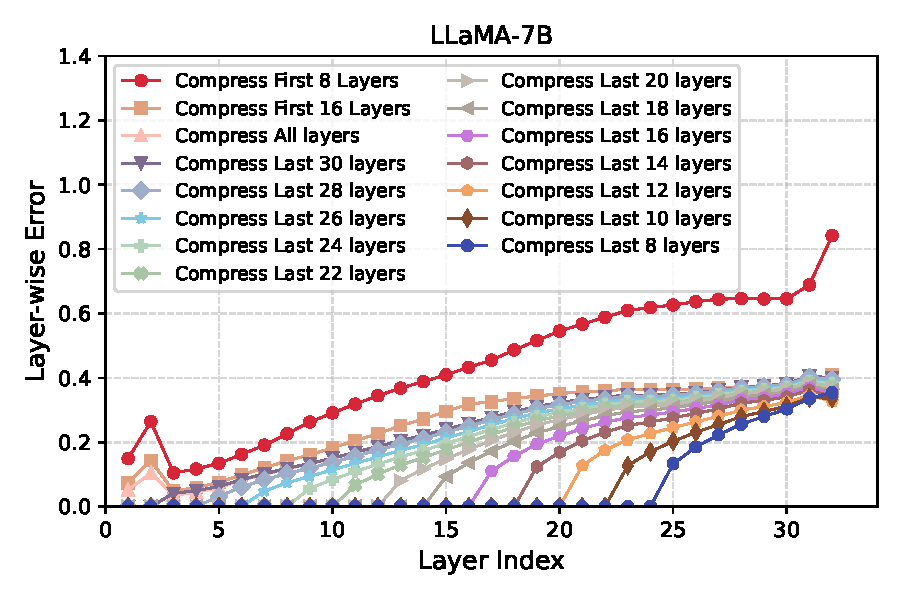
\includegraphics[width=\linewidth]{CPAL-2025-template/a_figures/llama_loss_comparison.pdf}
  \end{subfigure}
  % \hfill
  \begin{subfigure}[t]{0.49\linewidth}
    \centering
    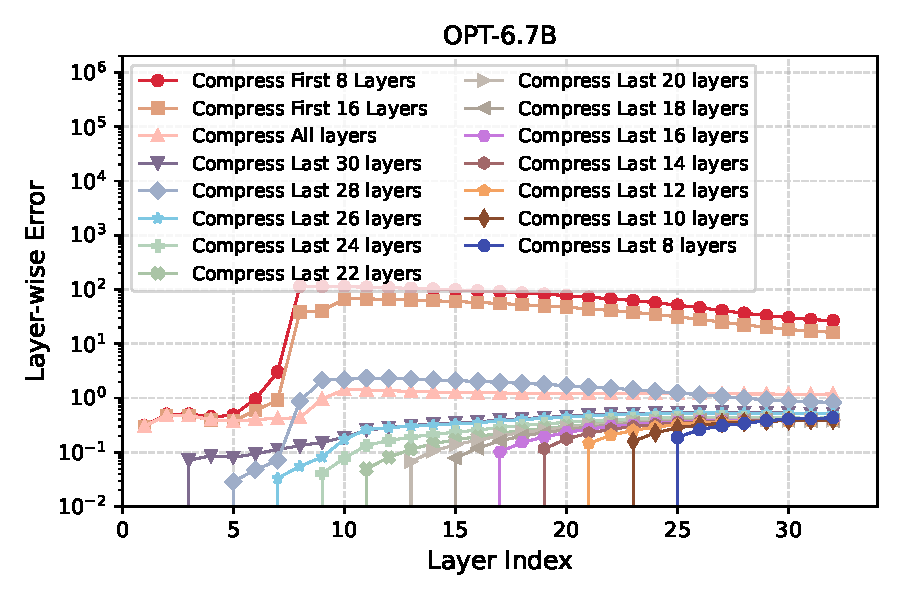
\includegraphics[width=\linewidth]{CPAL-2025-template/a_figures/opt_loss_comparison.pdf}
  \end{subfigure}

  \caption{
    Layer-wise error comparison between the original model, LLaMA-7B, and OPT-6.7B compressed by ERC-SVD with different layer selection strategies on WikiText-2. The overall compression ratio is 20\%, and all layer selection strategies strictly adhere to the compression constraint.
  }
  \label{layer-wise_error_comparison_llm}
\end{figure}
